\documentclass[DaoFP]{subfiles}
\begin{document}
 \setcounter{chapter}{10}

 \chapter{依赖类型 (Dependent Types)}

 我们已经见过依赖于其他类型的类型。它们是使用类型构造器和类型参数定义的,例如 \hask{Maybe} 或 \hask{[]}。大多数编程语言都支持泛型数据类型——即参数化的类型。

 在范畴论中,这类类型被建模为函子\footnote{没有 \hask{Functor} 实例的类型构造器可以被认为是来自离散范畴的函子——一个除了恒等箭头外没有其他箭头的范畴。}。

 一个自然的推广是定义依赖于值的类型。例如,将列表的长度编码到它的类型中通常是有利的。长度为零的列表将具有与长度为一的列表不同的类型,依此类推。

 显然,不能改变这种列表的长度,因为这会改变其类型。在函数式编程中,这不是问题,因为所有的数据类型都是不可变的。当向列表前面添加一个元素时,至少在概念上,会创建一个新的列表。对于长度编码的列表,新列表只是一个不同的类型!

 这些由值参数化的类型被称为\emph{依赖类型}。像 Idris 或 Agda 这样的语言完全支持依赖类型。在 Haskell 中也可以实现依赖类型,但对它们的支持仍然有限。

 在编程中使用依赖类型的原因是为了使程序在形式上是正确的。为了做到这一点,编译器必须能够检查程序员做出的假设。

 Haskell 以其强类型系统,能够在编译时揭示很多错误。例如,除非为变量的类型提供 \hask{Monoid} 实例,否则不会允许编写 \hask{a <> b}(\hask{mappend} 的中缀表示法)。

 然而,在 Haskell 的类型系统中,没有办法表达或更不用说强制执行幺半群的单位元和结合律。为了实现这一点,\hask{Monoid} 类型类的实例必须携带等式的证明(而不是实际的代码):
 \begin{haskell}
  assoc :: m <> (n <> p) = (m <> n) <> p
  lunit :: mempty <> m = m
  runit :: m <> mempty = m
 \end{haskell}
 依赖类型,特别是等式类型,为实现这一目标铺平了道路。

 本章的内容更加高级,并且在本书的其他部分中不会使用,因此您可以在第一次阅读时跳过。此外,为避免在纤维和函数之间产生混淆,我决定在本章的部分内容中使用大写字母表示对象。

 \section{依赖向量 (Dependent Vectors)}

 我们将从一个标准的例子开始,即计数列表或向量:
 \begin{haskell}
  data Vec n a where
  VNil  :: Vec Z a
  VCons :: a -> Vec n a -> Vec (S n) a
 \end{haskell}
 如果您包含以下语言声明,编译器将识别此定义为依赖类型:
 \begin{haskell}
 {-# LANGUAGE DataKinds #-}
 {-# LANGUAGE GADTs #-}
 \end{haskell}
 类型构造器的第一个参数是自然数 \hask{n}。请注意:这是一个值,而不是类型。类型检查器能够从数据构造器中 \hask{n} 的使用情况推断出来。第一个构造器创建类型为 \hask{Vec Z a} 的向量,第二个构造器创建类型为 \hask{Vec (S n) a} 的向量,其中 \hask{Z} 和 \hask{S} 被定义为自然数的构造器:
 \begin{haskell}
  data Nat = Z | S Nat
 \end{haskell}

 如果我们使用以下语言声明可以更明确地指定参数:
 \begin{haskell}
 {-# LANGUAGE KindSignatures #-}
 \end{haskell}
 并导入以下库:
 \begin{haskell}
  import Data.Kind
 \end{haskell}
 然后我们可以指定 \hask{n} 是一个 \hask{Nat},而 \hask{a} 是一个 \hask{Type}:
 \begin{haskell}
  data Vec (n :: Nat) (a :: Type) where
  VNil  :: Vec Z a
  VCons :: a -> Vec n a -> Vec (S n) a
 \end{haskell}

 使用这些定义之一,我们可以构造一个长度为零的整数向量:
 \begin{haskell}
  emptyV :: Vec Z Int
  emptyV = VNil
 \end{haskell}
 它的类型与长度为一的向量不同:
 \begin{haskell}
  singleV :: Vec (S Z) Int
  singleV = VCons 42 VNil
 \end{haskell}
 等等。

 我们现在可以定义一个依赖类型的函数,该函数返回向量的第一个元素:
 \begin{haskell}
  headV :: Vec (S n) a -> a
  headV (VCons a _) = a
 \end{haskell}
 此函数保证仅适用于非零长度的向量。这些是大小符合 \hask{(S n)} 的向量,这些向量不能是 \hask{Z}。如果尝试使用 \hask{emptyV} 调用此函数,编译器将会报错。

 另一个例子是将两个向量压缩在一起的函数。其类型签名中编码了两个向量的大小相同 \hask{n} 的要求(结果也是 \hask{n} 大小):
 \begin{haskell}
  zipV :: Vec n a -> Vec n b -> Vec n (a, b)
  zipV (VCons a as) (VCons b bs) = VCons (a, b) (zipV as bs)
  zipV VNil VNil = VNil
 \end{haskell}

 依赖类型在编码容器的形状时尤其有用。例如,列表的形状被编码为其长度。一个更高级的例子是在运行时将树的形状编码为值。

 \begin{exercise}
  实现函数 \hask{tailV},该函数返回非零长度向量的尾部。尝试使用 \hask{emptyV} 调用它。
 \end{exercise}

 \section{范畴上的依赖类型 (Dependent Types Categorically)}

 可视化依赖类型的最简单方法是将它们视为由集合的元素索引的类型族。在计数向量的情况下,索引集合是自然数集合 $\mathbb{N}$。

 第零个类型是表示空向量的单位类型 \hask{()}。与 \hask{(S Z)} 对应的类型是 \hask{a};然后我们有一个 \hask{(a, a)} 对,接下来是一个三元组 \hask{(a, a, a)},依此类推,随着 \hask{a} 的幂次增加。

 如果我们想将整个族视为一个大集合,我们可以取所有这些类型的和。例如,所有 \hask{a} 的幂次和是熟悉的列表类型,即自由幺半群:
 \[ \mathit{List} (a) = 1 + a + a \times a + a \times a \times a + \dots =  \sum_{n:\mathbb{N}} a^n \]

 \subsection{纤维 (Fibrations)}

 尽管直观上容易理解,但这种观点在推广到范畴论时效果不好,因为在范畴论中我们不喜欢将集合与对象混合。因此,我们将这个图景倒置,而不是谈论将族成员注入和中,我们考虑一个相反方向的映射。

 首先,我们可以再次使用集合来可视化这个过程。我们有一个大集合 $E$ 描述整个族,并有一个称为投影函数 $p$,或\index{display map}\emph{显示映射},该函数从 $E$ 映射到索引集 $B$(也称为\emph{基})。

 通常情况下,该函数将多个元素映射到一个元素。然后我们可以讨论某个特定元素 $x \in B$ 的逆映射作为 $p$ 映射到它的元素的集合。该集合称为\index{fiber}\emph{纤维},记作 $p^{-1} x$(尽管一般来说,$p$ 不是通常意义上的可逆函数)。将 $E$ 视为纤维的集合,$E$ 通常称为\emph{纤维丛}。

 \[
  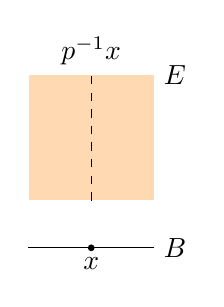
\begin{tikzpicture}

   \def\yb{0}; % base
   \def\yfb{0.6}; % fiber bottom
   \def\yft{2.2}; % fiber top

   \def\dx{0.8};

   \def\xbl{0};
   \def\xbm{\xbl + \dx};
   \def\xbr{\xbl + 2*\dx};

   \filldraw[fill=orange!30, draw=white] (\xbl, \yfb) rectangle (\xbr, \yft);

   \draw (\xbl, \yb) -- (\xbr, \yb);

   \draw[dashed] (\xbm, \yfb) -- (\xbm, \yft);

   \filldraw[black] (\xbm, \yb) circle (1 pt);
   \node[below] at (\xbm, \yb) {$x$};
   \node[above] at (\xbm, \yft) {$p^{-1} x$};
   \node[right] at (\xbr, \yb) {$B$};
   \node[right] at (\xbr, \yft) {$E$};

  \end{tikzpicture}
 \]

 现在我们暂时忘记集合的概念。在任意范畴中,\emph{纤维化} 是对象 $e$ 和 $b$ 以及箭头 $p \colon e \to b$ 的一个对。

 因此,这实际上只是一个箭头,但上下文至关重要。当箭头被称为纤维化时,我们使用集合的直觉,并将其源 $e$ 想象为一个纤维集合,其中 $p$ 将每个纤维投影到基 $b$ 中的一个点。

 我们甚至可以更进一步:由于(小)范畴形成一个以函子为箭头的范畴 $\mathbf{Cat}$,我们可以定义一个范畴的纤维化,并取另一个范畴作为其基。

 \subsection{作为纤维化的类型族 (Type Families as Fibrations)}

 因此,我们将类型族建模为纤维化。例如,我们的计数向量族可以表示为一个基为自然数类型的纤维化。整个族是连续幂次的和(上积)的并集:
 \[ \mathit{List}(a) = a^0 + a^1 + a^2 + \dots = \sum_{n\colon \mathbb{N}} a^n \]
 其中第零幂次——初始对象——表示大小为零的向量。
 \[
  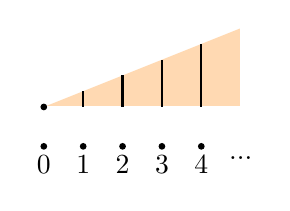
\begin{tikzpicture}
   \def\dx{0.5};
   \def\yb{0};
   \def\dy{0.2};
   \def\y{0.5};

   \filldraw[fill=orange!30, draw=white] (0, \y) to (5* \dx, \y) to (5*\dx, \y + 5*\dy);

   \filldraw[black] (0, 0) circle (1 pt);
   \node[below] at (0, 0) {$0$};
   \filldraw[black] (0, \y) circle (1 pt);

   \filldraw[black] (\dx, 0) circle (1 pt);
   \node[below] at (\dx, 0) {$1$};
   \draw[thick] (\dx, \y) -- (\dx, \y + \dy);

   \filldraw[black] (2*\dx, 0) circle (1 pt);
   \node[below] at (2*\dx, 0) {$2$};
   \draw[thick] (2*\dx, \y) -- (2*\dx, \y + 2* \dy);

   \filldraw[black] (3*\dx, 0) circle (1 pt);
   \node[below] at (3*\dx, 0) {$3$};
   \draw[thick] (3*\dx, \y) -- (3*\dx, \y + 3* \dy);

   \filldraw[black] (4*\dx, 0) circle (1 pt);
   \node[below] at (4*\dx, 0) {$4$};
   \draw[thick] (4*\dx, \y) -- (4*\dx, \y + 4* \dy);
   \node[below] at (5*\dx, 0) {$...$};

  \end{tikzpicture}
 \]

 投影 $p \colon \mathit{List}(a) \to \mathbb{N}$ 是熟悉的 $\mathit{length}$ 函数。

 在范畴论中,我们喜欢成批地描述事物——通过保持结构的映射定义事物的内部结构。纤维化就是这样一种情况。如果我们固定基对象 $b$ 并考虑范畴 $\mathcal{C}$ 中所有可能的源对象,以及所有可能的投影到 $b$ 的映射,我们得到一个\emph{商范畴} $\mathcal{C}/b$。这个范畴表示我们可以在基 $b$ 上切分范畴 $\mathcal{C}$ 的所有方式。

 回想一下,商范畴中的对象是对 $\langle e, p \colon e \to b \rangle$,而两个对象 $\langle e, p \rangle$ 和 $\langle e', p' \rangle$ 之间的态射是箭头 $f \colon e \to e'$,它与投影相通,即:
 \[p' \circ f = p \]
 最好通过注意到这种态射将 $p$ 的纤维映射到 $p'$ 的纤维来可视化这一点。这是一个“保持纤维”的丛之间的映射。

 \[
  \begin{tikzcd}
   e
   \arrow[rd, "p"']
   \arrow[rr, "f"]
   && e'
   \arrow[ld, "p'"]
   \\
   &b
  \end{tikzcd}
 \]

 我们的计数向量可以看作是商范畴 $\mathcal{C}/\mathbb{N}$ 中的对象,由对 $\langle \mathit{List}(a), \mathit{length} \rangle$ 组成。此范畴中的态射将长度为 $n$ 的向量映射为同样长度 $n$ 的向量。

 \subsection{纤维化的拉回 (Pullbacks)}

 我们见过许多通方格的例子。这样的方格是一个等式的图形表示:两个路径连接方格的对角,每个路径都是两个态射组成的结果是相等的。

 如同每个等式一样,我们可能希望用一个或多个未知量替换其组成部分,并尝试解决所得到的等式。例如,我们可以问:是否有一个对象与两个箭头一起能完成一个通方格?如果存在许多这样的对象,是否有一个是通用的?如果缺少拼图的部分是方格的左上角(源),我们称之为拉回(pullback)。如果是右下角(目标),我们称之为\index{pushout}推送(pushout)。

 \[
  \begin{tikzcd}
   \color{red}?
   \arrow[d, red, dashed, "?"']
   \arrow[r, red, dashed, "?"]
   & E
   \arrow[d, "p"]
   \\
   A
   \arrow[r, "f"]
   &B
  \end{tikzcd}
  \hspace{40pt}
  \begin{tikzcd}
   E
   \arrow[d, "p"']
   \arrow[r, "f"]
   & E'
   \arrow[d, red, dashed, "?"]
   \\
   B
   \arrow[r, red, dashed, "?"]
   &\color{red}?
  \end{tikzcd}
 \]

 让我们从一个特定的纤维化 $p \colon E \to B$ 开始,问问自己:当我们将基从 $B$ 更改为通过映射 $f \colon A \to B$ 相关的某个 $A$ 时,会发生什么?我们能否沿着 $f$ “将纤维拉回”?

 再次,我们先考虑集合。想象在 $E$ 中选取一个纤维,在 $B$ 中某个点 $y$ 上方,该点属于 $f$ 的像。若 $f$ 是可逆的,则会有一个元素 $x = f^{-1} y$。我们会将纤维植入它的上方。然而,一般来说,$f$ 不是可逆的。这意味着可能有多个 $A$ 的元素映射到我们的 $y$。在下面的图中,您会看到两个这样的元素,$x_1$ 和 $x_2$。我们只需将纤维克隆并植入所有映射到 $y$ 的元素上。这种方式,每个 $A$ 中的点都会有一个纤维从它生长出来。所有这些纤维的总和将形成一个新的纤维丛 $E'$。

 \[
  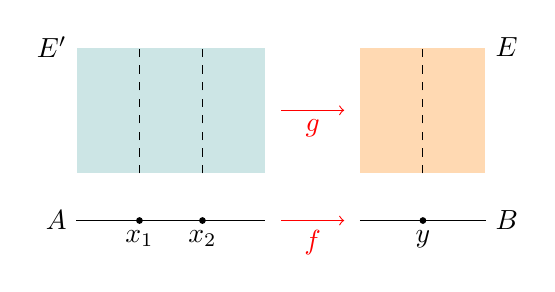
\begin{tikzpicture}

   \def\yb{0}; % base
   \def\yfb{0.6}; % fiber bottom
   \def\yft{2.2}; % fiber top
   \def\yfm{1.4} % fiber middle

   \def\dx{0.8};

   \def\xal{-1.8};
   \def\xam{\xal + \dx};
   \def\xamm{\xal + 2 * \dx};
   \def\xar{\xal + 3*\dx};

   \def\xbl{1.8};
   \def\xbm{\xbl + \dx};
   \def\xbr{\xbl + 2*\dx};

   \filldraw[fill=blue!50!green!20, draw=white] (\xal, \yfb) rectangle (\xar, \yft);
   \filldraw[fill=orange!30, draw=white] (\xbl, \yfb) rectangle (\xbr, \yft);

   \draw (\xal, \yb) -- (\xar, \yb);
   \draw (\xbl, \yb) -- (\xbr, \yb);

   \draw[dashed] (\xam, \yfb) -- (\xam, \yft);
   \draw[dashed] (\xamm, \yfb) -- (\xamm, \yft);
   \draw[dashed] (\xbm, \yfb) -- (\xbm, \yft);

   \filldraw[black] (\xam, \yb) circle (1 pt);
   \filldraw[black] (\xamm, \yb) circle (1 pt);
   \filldraw[black] (\xbm, \yb) circle (1 pt);
   \node[below] at (\xbm, \yb) {$y$};
   \node[right] at (\xbr, \yb) {$B$};
   \node[left] at (\xal, \yb) {$A$};
   \node[right] at (\xbr, \yft) {$E$};
   \node[left] at (\xal, \yft) {$E'$};
   \node[below] at (\xam, \yb) {$x_1$};
   \node[below] at (\xamm, \yb) {$x_2$};

   \draw[->, red] (\xar + 0.2, \yb) -- (\xbl - 0.2, \yb) node [midway, below] {$f$};
   \draw[->, red] (\xar + 0.2, \yfm) -- (\xbl - 0.2, \yfm) node [midway, below] {$g$};

  \end{tikzpicture}
 \]

 因此我们构造了一个基为 $A$ 的新纤维化。其投影 $p' \colon E' \to A$ 将每个点映射到其纤维被植入的点上。还有一个明显的映射 $g \colon E' \to E$,它将纤维映射到相应的纤维。

 通过构造,这个新的纤维化 $\langle E', p'\rangle$ 满足条件:
 \[ p \circ g = f \circ p' \]
 它可以表示为一个通方格:
 \[
  \begin{tikzcd}
   E'
   \arrow[d, "p'"']
   \arrow[r, "g"]
   & E
   \arrow[d, "p"]
   \\
   A
   \arrow[r, "f"]
   &B
  \end{tikzcd}
 \]

 在 $\mathbf{Set}$ 中,我们可以将 $E'$ 显式构造为笛卡尔积 $A \times E$ 的\emph{子集},其中 $p' = \pi_1$,$g = \pi_2$(两个笛卡尔投影)。$E'$ 的元素是满足条件 $f (a) = p (e)$ 的对 $\langle a, e \rangle$。

 这个通方格是范畴论推广的起点。然而,即使在 $\mathbf{Set}$ 中,仍然存在许多不同的 $A$ 上方的纤维化,它们使该图表通方。我们必须选择通用的那个。这样的通用构造称为\emph{拉回},或称为\emph{纤维积}。

 在范畴论中,$p \colon e \to b$ 沿着 $f \colon a \to b$ 的拉回是一个对象 $e'$ 和两个箭头 $p' \colon e' \to a$ 和 $g \colon e' \to e$,它们使以下图表通方:
 \[
  \begin{tikzcd}
   &e'
   \arrow[r, "g"]
   \arrow[d, "p'"']
   &e
   \arrow[d, "p"]
   \\
   &a
   \arrow[r, "f"]
   &b
  \end{tikzcd}
 \]
 并满足通用条件。

 通用条件表明,对于任何其他候选对象 $x$,它有两个箭头 $q' \colon x \to e$ 和 $q \colon x \to a$,使得 $p \circ q' = f \circ q$(使大“方格”通方),存在一个唯一的箭头 $h \colon x \to e'$,使得两个三角形通方,即:
 \begin{align*}
  q &= p' \circ h \\
  q' &= g \circ h
 \end{align*}
 图形表示如下:
 \[
  \begin{tikzcd}
   x
   \arrow[dr, dashed, "h"]
   \arrow[drr, bend left, "q'"]
   \arrow[ddr, bend right, "q"']
   \\
   &e'
   \arrow[r, "g"]
   \arrow[d, "p'"']
   \arrow[dr, phantom,  , very near start, "\lrcorner"]
   &e
   \arrow[d, "p"]
   \\
   &a
   \arrow[r, "f"]
   &b
  \end{tikzcd}
 \]
 方格的上角的角度符号用于标记拉回。

 如果我们通过集合和纤维的视角来看拉回,$e$ 是 $b$ 上的纤维丛,而我们正在从 $e$ 中的纤维构造一个新的纤维丛。将这些纤维植入 $a$ 上的位置由 $f$ 的逆像决定。此过程使得 $e'$ 成为 $a$ 和 $b$ 上的纤维丛,后者的投影为 $p \circ g = f \circ p'$。

 这个图中的 $x$ 是某个 $a$ 上的其他纤维丛,其投影为 $q$。它同时也是一个 $b$ 上的纤维丛,其投影为 $f \circ q = p \circ q'$。唯一的映射 $h$ 将 $q^{-1}$ 给出的 $x$ 的纤维映射到 $p'^{-1}$ 给出的 $e'$ 的纤维。

 这个图中的所有映射都作用在纤维上。有些映射重新排列纤维到新的基上——这是拉回的作用。其他映射修改单个纤维——映射 $h \colon x \to e'$ 这样工作。

 如果您将纤维丛视为纤维的容器,纤维的重新排列对应于自然变换,而纤维的修改对应于 \hask{fmap} 的作用。

 然后通用条件告诉我们,$q'$ 可以分解为纤维的修改 $h$,然后是纤维的重新排列 $g$。

 值得注意的是,选择终对象或单元素集合作为拉回目标会自动给出笛卡尔积的定义:
 \[
  \begin{tikzcd}
   b \times e
   \arrow[d, "\pi_1"']
   \arrow[r, "\pi_2"]
   \arrow[dr, phantom,  , very near start, "\lrcorner"]
   & e
   \arrow[d, "!"]
   \\
   b
   \arrow[r, "!"]
   &
   1
  \end{tikzcd}
 \]

 或者,我们可以将这个图看作是将尽可能多的 $e$ 的副本种植到 $b$ 的每个元素上。当我们谈论依赖和积时,我们将使用这个类比。

 还请注意,可以通过将其拉回到终对象来从纤维化中提取单个纤维。在这种情况下,映射 $x \colon 1 \to b$ 选择了基的一个元素,沿着它的拉回提取单个纤维 $\varphi$:
 \[
  \begin{tikzcd}
   \varphi
   \arrow[d, "!"']
   \arrow[r, "g"]
   \arrow[dr, phantom,  , very near start, "\lrcorner"]
   & e
   \arrow[d, "p"]
   \\
   1
   \arrow[r, "x"]
   &
   b
  \end{tikzcd}
 \]
 箭头 $g$ 将该纤维注入回 $e$。通过更改 $x$ 我们可以选择 $e$ 中的不同纤维。

 \begin{exercise}
  证明终对象作为目标的拉回就是乘积。
 \end{exercise}
 \begin{exercise}
  证明可以将拉回定义为棒形范畴的图的极限,该范畴有三个对象:
  \[ a \rightarrow b \leftarrow c \]
 \end{exercise}

 \begin{exercise}
  证明 $b$ 作为目标的 $\mathcal{C}$ 中的拉回是商范畴 $\mathcal{C}/b$ 中的乘积。提示:定义两个投影作为商范畴中的态射。使用拉回的通用性来证明乘积的通用性。
 \end{exercise}

 \subsection{替换 (Substitution)}

 我们有两种描述依赖类型的替代方法:一种是作为纤维化,另一种是作为类型族。在后一种框架中,沿着态射 $f$ 的拉回可以解释为替换。当我们有一个由元素 $y \colon B$ 参数化的类型族 $T y$ 时,我们总是通过将 $f x$ 替换为 $y$ 来定义一个新的类型族。

 \[
  \begin{tikzcd}
   T (f x)
   & T y
   \\
   x
   \arrow[u, mapsto, ""]
   \arrow[r, mapsto, "f"]
   &y
   \arrow[u, mapsto, ""]
  \end{tikzcd}
 \]
 因此,新的类型族由不同的形状参数化。

 \subsection{依赖环境 (Dependent Environments)}
 在建模 lambda 演算时,我们使用笛卡尔闭范畴的对象同时作为类型和环境。空环境被建模为终对象(单位类型),我们使用乘积构建更复杂的环境。由于乘积在同构(up to isomorphism)下是对称的,乘积类型的顺序无关紧要。

 处理依赖类型时,我们必须考虑到添加到环境中的类型可能取决于环境中已经存在的类型的值。如前所述,我们从终对象表示的空环境开始。

 \subsection{弱化 (Weakening)}

 \subsection{基变换函子 (Base-Change Functor)}

 我们使用笛卡尔闭范畴作为编程的模型。要建模依赖类型,我们需要施加一个附加条件:我们要求范畴是\index{locally cartesian closed category}\emph{局部笛卡尔闭范畴}。这是一个所有商范畴都是笛卡尔闭的范畴。

 特别地,这种范畴具有所有拉回,因此始终可以更改任何纤维化的基。基变换在商范畴之间引入一个函子的映射。

 给定两个商范畴 $\mathcal{C}/b$ 和 $\mathcal{C}/a$ 以及一个基之间的箭头 $f \colon b \to a$,基变换函子 $f^* \colon \mathcal{C}/a \to \mathcal{C}/b$ 将纤维化 $\langle e, p \rangle$ 映射到纤维化 $ f^* \langle e, p \rangle= \langle f^* e, f^* p \rangle$,该纤维化由拉回给出:
 \[
  \begin{tikzcd}
   f^* e
   \arrow[dr, phantom,  , very near start, "\lrcorner"]
   \arrow[d, "f^*p"']
   \arrow[r, "g"]
   & e
   \arrow[d, "p"]
   \\
   b
   \arrow[r, "f"]
   &a
  \end{tikzcd}
 \]
 请注意,函子 $f^*$ 的方向与箭头 $f$ 的方向相反。

 为了可视化基变换函子,让我们考虑它如何作用于集合。
 \[
  \begin{tikzcd}
   f^* E
   \arrow[dr, phantom,  , very near start, "\lrcorner"]
   \arrow[d, "f^*p"']
   \arrow[r, "g"]
   & E
   \arrow[d, "p"]
   \\
   B
   \arrow[r, "f"]
   &A
  \end{tikzcd}
 \]
 我们有一个直觉,即纤维化 $p$ 将集合 $E$ 分解为每个 $A$ 点上的纤维。

 我们可以将 $f$ 视为另一个纤维化,以类似方式分解 $B$。我们将 $B$ 中的纤维称为“片”。例如,如果 $A$ 是一个两元素集合,那么由 $f$ 给出的纤维化将 $B$ 分成两个片。拉回则将 $E$ 的纤维拉回并将其植入 $B$ 中的每个片中。结果集 $f^*E$ 看起来像一个拼布,其中每个片都种植了 $E$ 的单个纤维的克隆。

 \[
  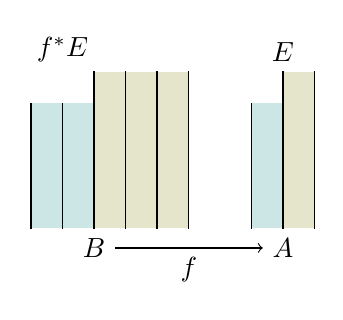
\begin{tikzpicture}
   \def\xmin{1.4};
   \def\dx{0.4};
   \def\xl{-1.4};

   \def\dy{0.2};
   \def\yb{0};
   \def\yt{10 * \dy};

% bars over A
   \filldraw[fill=blue!50!green!20, draw=white] (\xmin, \yb) rectangle (\xmin + \dx, \yt - 2*\dy);
   \filldraw[fill=red!50!green!20, draw=white] (\xmin + \dx, \yb) rectangle (\xmin + 2 * \dx, \yt);

   \draw (\xmin, \yb) -- (\xmin, \yt - 2*\dy);
   \draw (\xmin + \dx, \yb) -- (\xmin+ \dx, \yt);
   \draw (\xmin + 2 * \dx, \yb) -- (\xmin + 2 * \dx, \yt);

   \node[below] (BB) at (\xmin + \dx, \yb) {$A$};
   \node[above] at (\xmin + \dx, 10 * \dy) {$E$};

% bars over B

   \filldraw[fill=blue!50!green!20, draw=white] (\xl, \yb) rectangle (\xl + 5 * \dx, \yt - 2*\dy);
   \filldraw[fill=red!50!green!20, draw=white] (\xl + 2*\dx, \yb) rectangle (\xl + 5 * \dx, \yt);
   \draw (\xl, \yb) -- (\xl, \yt - 2*\dy);
   \draw (\xl + \dx, \yb) -- (\xl + \dx, \yt - 2 * \dy);
   \draw (\xl + 2 * \dx, \yb) -- (\xl + 2 * \dx, \yt);
   \draw (\xl + 3 * \dx, \yb) -- (\xl + 3 * \dx, \yt);
   \draw (\xl + 4 * \dx, \yb) -- (\xl + 4 * \dx, \yt);
   \draw (\xl + 5 * \dx, \yb) -- (\xl + 5 * \dx, \yt);

   \node[below] (B) at (\xl + 2 * \dx, \yb) {$B$};
   \node[above] at (\xl + \dx, 10 * \dy) {$f^* E$};

   \draw[->]  (B) -- (BB) node [midway, below] {$f$};


  \end{tikzpicture}
 \]

 由于我们有一个从 $B$ 到 $A$ 的函数,可能会将多个元素映射为一个,因此 $B$ 上的纤维化比 $A$ 上的纤维化更精细。将 $E$ 在 $A$ 上的纤维化转变为在 $B$ 上的纤维化的最简单、最省力的方式是将现有的纤维扩展到($f$ 的逆像定义的)片。这是拉回的通用构造的本质。

 特别地,如果 $A$ 是一个单元素集合(终对象),那么我们只有一个纤维(整个 $E$),丛 $f^*E$ 是一个笛卡尔积 $B \times E$。这样的丛称为\index{trivial bundle}\emph{平凡丛}。

 非平凡丛不是积,但可以\emph{局部}分解为积。正如 $B$ 是片的和,$f^*E$ 是这些片与 $E$ 的相应纤维的积的和。

 您还可以将 $A$ 视为提供了一个枚举基 $B$ 中所有片的\emph{地图集}。想象 $A$ 是一组国家,而 $B$ 是一组城市。映射 $f$ 为每个城市指定一个国家。

 继续这个例子,让 $E$ 是由国家纤维化的语言集。如果我们假设在每个城市中都讲该国的语言,那么基变换函子将国家的语言重新植入其每个城市。

 顺便提一下,这种使用局部片和地图集的思想可以追溯到微分几何和广义相对论,我们经常将局部坐标系粘合在一起,以描述拓扑上非平凡的丛,如莫比乌斯带或克莱因瓶。

 正如我们很快将看到的那样,在局部笛卡尔闭范畴中,基变换函子同时具有左伴随和右伴随。$f^*$ 的左伴随称为 $f_!$(有时发音为“f 下惊叹号”),右伴随称为 $f_*$(“f 下星号”):
 \[ f_! \dashv f^* \dashv f_* \]
 在编程中,左伴随称为依赖和,右伴随称为依赖积或依赖函数:
 \[ \Sigma_f \dashv f^* \dashv \Pi_f \]

 \begin{exercise}
  定义基变换函子对 $\cat C/a$ 中态射的作用,即给定一个态射 $h$,构造其对映 $f^* h$。
  \[
   \begin{tikzcd}
    f^* e'
    \arrow[dr, "f^*p'"']
    \arrow[r, red, "f^* h"]
    & f^* e
    \arrow[d, "f^*p"]
    && e'
    \arrow[d, "p'"]
    \arrow[r, red, "h"]
    & e
    \arrow[dl, "p"]
    \\
    & b
    \arrow[rr, "f"']
    &&a
   \end{tikzcd}
   \hspace{40pt}
   \begin{tikzcd}
   \end{tikzcd}
  \]
  提示:使用拉回的通用性和通方条件:$g' \circ h \circ p = f^* p' \circ f$。

  \[
   \begin{tikzcd}
    f^* e'
    \arrow[dr, dashed, red, "f^* h"]
    \arrow[drr, bend left, "g' \circ h"]
    \arrow[ddr, bend right, "f^* p'"']
    \\
    &f^* e
    \arrow[r, "g"]
    \arrow[d, "f^* p"']
    \arrow[dr, phantom,  , very near start, "\lrcorner"]
    &e
    \arrow[d, "p"]
    \\
    &b
    \arrow[r, "f"]
    &a
   \end{tikzcd}
   \hspace{40pt}
   \begin{tikzcd}
    f^* e'
    \arrow[r, "g'"]
    \arrow[d, "f^* p'"']
    \arrow[dr, phantom,  , very near start, "\lrcorner"]
    & e'
    \arrow[d, "p'"']
    \arrow[r, red, "h"]
    & e
    \arrow[dl, "p"]
    \\
    b
    \arrow[r, "f"]
    & a
   \end{tikzcd}
  \]

 \end{exercise}


  \section{依赖和 (Dependent Sum)}

  在类型理论中,依赖和,或 sigma 类型 $\Sigma_{x : B} T(x)$,定义为一对元素的类型,其中第二个元素的\emph{类型}依赖于第一个元素的\emph{值}。

  从概念上讲,和类型通过其映射出性质(mapping-out property)定义。和的映射出是一个对映,如下的伴随关系所示:
  \[ \mathcal{C}(F_1 + F_2, F) \cong (\mathcal{C} \times \mathcal{C}) (\langle F_1, F_2 \rangle, \Delta F) \]
  在这里,我们有一对箭头 $(F_1 \to F, F_2 \to F)$,它们定义了和 $S = F_1 + F_2$ 的映射出。在 $\Set$ 中,和是带标签的并集。依赖和是由另一个集合的元素标记的和。

  我们的计数向量类型可以被认为是由自然数标记的依赖和。这种类型的元素是一个自然数 \hask{n}(一个值)与一个 n 元组类型 \hask{(a, a, ... a)} 的元素配对。以下是一些用这种表示法编写的整数计数向量:
  \begin{haskell}
   (0, ())
   (1, 42)
   (2, (64, 7))
   (5, (8, 21, 14, -1, 0))
  \end{haskell}

  更一般地说,依赖和的引入规则假设存在一个由基类型 $B$ 的元素索引的类型族 $T(x)$。然后 $\Sigma_{x : B} T(x)$ 的元素由一对元素 $x \colon B$ 和 $y \colon T(x)$ 构成。

  从范畴论的角度看,依赖和被建模为基变换函子的左伴随。

  为了理解这一点,我们首先回顾一下积的定义,它是积的元素。我们之前已经注意到,积可以表示为从单元素集合(终对象)拉回的积。以下是积/拉回的通用构造(符号表示了该构造的目标):
  \[
   \begin{tikzcd}
    S
    \arrow[dr, blue, dashed, "\phi^T"]
    \arrow[drr, blue, bend left, "\phi"]
    \arrow[ddr, bend right, "q"]
    \\
    &B \times F
    \arrow[dr, phantom,  , very near start, "\lrcorner"]
    \arrow[r, "\pi_2"]
    \arrow[d, "\pi_1"']
    &F
    \arrow[d, "!"]
    \\
    &B
    \arrow[r, "!"]
    &1
   \end{tikzcd}
  \]

  我们还看到积可以通过伴随关系来定义。我们可以在图中发现这种伴随关系:对于每一对箭头 $\langle \phi, q \rangle$,都有一个唯一的箭头 $\phi^T$ 使得三角形是可交换的。

  请注意,如果我们固定 $q$,我们会在箭头 $\phi$ 和 $\phi^T$ 之间得到一一对应的关系。这就是我们感兴趣的伴随关系。

  现在,我们可以戴上纤维化的眼镜,注意到 $\langle S, q\rangle$ 和 $\langle B \times F, \pi_1 \rangle$ 是在相同基 $B$ 上的两个纤维化。交换三角形使 $\phi^T$ 成为商范畴 $\mathcal{C}/B$ 中的一个态射,或者说是纤维间的映射。换句话说,$\phi^T$ 是同态集的一个成员:
  \[ (\mathcal{C}/B) \left(\left \langle {S \atop q} \right \rangle, \left \langle {B \times F \atop \pi_1} \right \rangle \right)  \]

  由于 $\phi$ 是同态集 $ \mathcal{C}(S, F)$ 的一个成员,我们可以将 $\phi^T$ 和 $\phi$ 之间的一一对应关系重写为同态集的同构:
  \[  (\mathcal{C}/B)\left(\left \langle {S \atop q} \right \rangle, \left \langle {B \times F \atop \pi_1} \right \rangle \right) \cong \mathcal{C}(S, F) \]
  实际上,这是一个伴随关系,其中我们有一个遗忘函子 $U \colon \mathcal{C}/B \to \mathcal{C}$,它将 $\langle S, q \rangle$ 映射到 $S$,从而遗忘了纤维化。

  如果你仔细看这个伴随关系,你可以看到将 $S$ 定义为范畴和(即余积)的轮廓。

  首先,在右边你有一个 $S$ 的映射出。将 $S$ 视为由纤维化 $\langle S, q \rangle$ 定义的纤维的和。

  其次,回想一下纤维化 $\langle B \times F, \pi_1 \rangle$ 可以被视为在 $B$ 的点上植入许多 $F$ 的副本。这是对对角函子 $\Delta$ 的推广,它复制 $F$,在这里,我们制作了“$B$ 副本”的 $F$。伴随关系的左侧只是一些箭头,每个箭头将 $S$ 的不同纤维映射到目标纤维 $F$。

  \[
   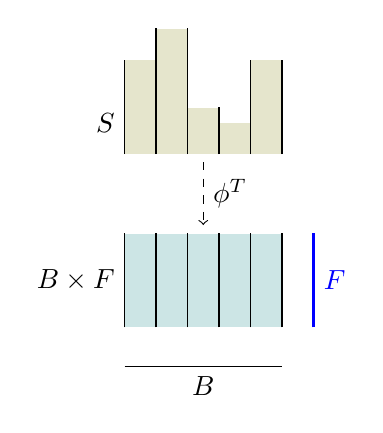
\begin{tikzpicture}
    \def\xmin{1.4};
    \def\dx{0.4};
    \def\xl{-1.4};

    \def\dy{0.2};
    \def\yb{0.2};
    \def\yt{10 * \dy};

    \def\ybb{-2};
    \def\ytt{\ybb + 6 * \dy};

    \def\ybase{-2.5}

% bars above

    \def\yya{\yt - 3 * \dy}
    \def\yyb{\yt - 1 * \dy}
    \def\yyc{\yt - 6 * \dy}
    \def\yyd{\yt - 7 * \dy}

    \filldraw[fill=red!50!green!20, draw=white] (\xl + 0*\dx, \yb) rectangle (\xl + 1 * \dx, \yya);
    \filldraw[fill=red!50!green!20, draw=white] (\xl + 1*\dx, \yb) rectangle (\xl + 2 * \dx, \yyb);
    \filldraw[fill=red!50!green!20, draw=white] (\xl + 2*\dx, \yb) rectangle (\xl + 3 * \dx, \yyc);
    \filldraw[fill=red!50!green!20, draw=white] (\xl + 3*\dx, \yb) rectangle (\xl + 4 * \dx, \yyd);
    \filldraw[fill=red!50!green!20, draw=white] (\xl + 4*\dx, \yb) rectangle (\xl + 5 * \dx, \yya);

    \draw (\xl + 0 * \dx, \yb) -- (\xl + 0 * \dx, \yya);
    \draw (\xl + 1 * \dx, \yb) -- (\xl + 1 * \dx, \yyb);
    \draw (\xl + 2 * \dx, \yb) -- (\xl + 2 * \dx, \yyb);
    \draw (\xl + 3 * \dx, \yb) -- (\xl + 3 * \dx, \yyc);
    \draw (\xl + 4 * \dx, \yb) -- (\xl + 4 * \dx, \yya);
    \draw (\xl + 5 * \dx, \yb) -- (\xl + 5 * \dx, \yya);


% bars below

    \filldraw[fill=blue!50!green!20, draw=white] (\xl, \ybb) rectangle (\xl + 5 * \dx, \ytt);
    \draw (\xl + 0 * \dx, \ybb) -- (\xl + 0 * \dx, \ytt);
    \draw (\xl + 1 * \dx, \ybb) -- (\xl + 1 * \dx, \ytt);
    \draw (\xl + 2 * \dx, \ybb) -- (\xl + 2 * \dx, \ytt);
    \draw (\xl + 3 * \dx, \ybb) -- (\xl + 3 * \dx, \ytt);
    \draw (\xl + 4 * \dx, \ybb) -- (\xl + 4 * \dx, \ytt);
    \draw (\xl + 5 * \dx, \ybb) -- (\xl + 5 * \dx, \ytt);

    \node[left] at (\xl, \ybb + 3 * \dy) {$B \times F$};
    \node[left] at (\xl, 3 * \dy) {$S$};
    \draw[thick, blue] (\xl + 6 * \dx, \ybb) -- (\xl + 6 * \dx, \ytt) node[midway, right] {$F$};
    \draw[] (\xl, \ybase) -- (\xl + 5 * \dx, \ybase) node [midway, below] {$B$};

    \draw[->, dashed] (\xl + 2.5 * \dx, \yb - 0.1) -- (\xl + 2.5 * \dx, \ytt + 0.1) node[midway, right] {$\phi^T$};

   \end{tikzpicture}
  \]

  将这一思想应用到我们的计数向量示例中,$\phi^T$ 代表无限多个函数,每个自然数一个。在实践中,我们使用递归来定义这些函数。例如,这里有一个整数向量的映射:
  \begin{haskell}
   sumV :: Vec n Int -> Int
   sumV VNil = 0
   sumV (VCons n v) = n + sumV v
  \end{haskell}

  \subsection{添加图集 (Adding the atlas)}

  我们可以通过用任意基 $A$(图集)替换终对象来推广我们的图表。现在,我们有了一个纤维化 $\langle F, p \rangle$,并且我们使用定义基变换函子 $f^*$ 的拉回方形:
  \[
   \begin{tikzcd}
    S
    \arrow[dr, blue, dashed, "\phi^T"]
    \arrow[drr, blue, bend left, "\phi"]
    \arrow[ddr, bend right, "q"]
    \\
    &f^* F
    \arrow[dr, phantom,  , very near start, "\lrcorner"]
    \arrow[r, "g"]
    \arrow[d, "f^* p"']
    &F
    \arrow[d, "p"]
    \\
    &B
    \arrow[r, "f"]
    &A
   \end{tikzcd}
  \]

  我们可以想象在 $B$ 上的纤维化更细粒度,因为 $f$ 可能将多个点映射到一个点。例如,考虑一个函数 \hask{even :: Nat -> Bool},它创建了偶数和奇数的两个集合。在此图中,$f$ 定义了对原始 $S$ 的粗略“重采样”。

  拉回的通用性导致了以下同态集的同构:

  \[  (\mathcal{C}/B) \left( \left \langle {S \atop q} \right \rangle , f^* \left \langle {F \atop p} \right \rangle \right) \cong (\mathcal{C}/A) \left( \left \langle {S \atop f \circ q } \right \rangle , \left \langle {F \atop p} \right \rangle \right)  \]
  在这里,$\phi^T$ 是左侧的一个元素,而 $\phi$ 是对应的右侧元素。

  我们将这个同构解释为基变换函子 $f^*$ 和依赖和函子之间的伴随关系。
  \[  (\mathcal{C}/B) \left( \left \langle {S \atop q} \right \rangle , f^* \left \langle {F \atop p} \right \rangle \right) \cong (\mathcal{C}/A) \left( \Sigma_f \left \langle {S \atop q} \right \rangle , \left \langle {F \atop p} \right \rangle \right)  \]
  依赖和因此由以下公式给出:
  \[ \Sigma_f \left \langle {S \atop q} \right \rangle =  \left \langle {S \atop f \circ q} \right \rangle \]
  这意味着,如果 $S$ 是通过 $q$ 在 $B$ 上纤维化的,并且存在从 $B$ 到 $A$ 的映射 $f$,那么 $S$ 就会自动(更粗略地)在 $A$ 上纤维化,投影为组合 $f \circ q$。

  我们之前已经看到,在 $\mathbf{Set}$ 中,$f$ 定义了 $B$ 内的补丁。$F$ 的纤维被重新植入这些补丁中,形成 $f^*F$。局部而言,即在每个补丁内,$f^*F$ 看起来像是一个笛卡尔积。

  \[
   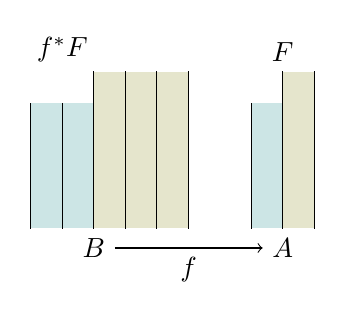
\begin{tikzpicture}
    \def\xmin{1.4};
    \def\dx{0.4};
    \def\xl{-1.4};

    \def\dy{0.2};
    \def\yb{0};
    \def\yt{10 * \dy};

% bars over A
    \filldraw[fill=blue!50!green!20, draw=white] (\xmin, \yb) rectangle (\xmin + \dx, \yt - 2*\dy);
    \filldraw[fill=red!50!green!20, draw=white] (\xmin + \dx, \yb) rectangle (\xmin + 2 * \dx, \yt);

    \draw (\xmin, \yb) -- (\xmin, \yt - 2*\dy);
    \draw (\xmin + \dx, \yb) -- (\xmin+ \dx, \yt);
    \draw (\xmin + 2 * \dx, \yb) -- (\xmin + 2 * \dx, \yt);

    \node[below] (BB) at (\xmin + \dx, \yb) {$A$};
    \node[above] at (\xmin + \dx, 10 * \dy) {$F$};

% bars over B

    \filldraw[fill=blue!50!green!20, draw=white] (\xl, \yb) rectangle (\xl + 5 * \dx, \yt - 2*\dy);
    \filldraw[fill=red!50!green!20, draw=white] (\xl + 2*\dx, \yb) rectangle (\xl + 5 * \dx, \yt);
    \draw (\xl, \yb) -- (\xl, \yt - 2*\dy);
    \draw (\xl + \dx, \yb) -- (\xl + \dx, \yt - 2 * \dy);
    \draw (\xl + 2 * \dx, \yb) -- (\xl + 2 * \dx, \yt);
    \draw (\xl + 3 * \dx, \yb) -- (\xl + 3 * \dx, \yt);
    \draw (\xl + 4 * \dx, \yb) -- (\xl + 4 * \dx, \yt);
    \draw (\xl + 5 * \dx, \yb) -- (\xl + 5 * \dx, \yt);

    \node[below] (B) at (\xl + 2 * \dx, \yb) {$B$};
    \node[above] at (\xl + \dx, 10 * \dy) {$f^* F$};

    \draw[->]  (B) -- (BB) node [midway, below] {$f$};


   \end{tikzpicture}
  \]
  $S$ 本身以两种方式纤维化:使用 $f \circ q$ 在 $A$ 上粗略地分割,并使用 $q$ 在 $B$ 上精细地切片。

  在范畴论中,依赖和是基变换函子 $f^*$ 的左伴随,记作 $f_!$。对于给定的 $f \colon b \to a$,这是一个函子:
  \[ f_! \colon \cat C/b \to \cat C/a \]
  它对对象 $(s, q \colon s \to b)$ 的作用由后组合 $f$ 给出:
  \[ f_! (s, q)= (s, f \circ q) \]

  \subsection{存在量化 (Existential quantification)}

  在“命题即类型”的解释中,类型族对应于命题族。依赖和类型 $\Sigma_{x : B} \, T(x)$ 对应于命题:存在一个 $x$ 使得 $T(x)$ 为真:
  \[ \exists_{x : B} \, T (x)\]

  确实,类型 $\Sigma_{x : B} \, T(x)$ 的一个术语是一个元素对,一个是 $x \colon B$,另一个是 $y \colon T(x)$——这表明 $T(x)$ 对于某个 $x$ 是可居住的。

  \section{依赖积 (Dependent Product)}

  在类型理论中,依赖积,或依赖函数,或 $\Pi$-类型 $\Pi_{x:B} T(x)$,定义为返回\emph{类型}取决于其参数的\emph{值}的函数。

  它被称为函数,因为你可以对其进行求值。给定一个依赖函数 $f \colon \Pi_{x:B} T(x)$,你可以将其应用于参数 $x\colon B$ 以获得 $f(x) \colon T(x)$ 的值。

  \subsection{Haskell 中的依赖积}
  一个简单的依赖积示例是一个构造具有给定大小的向量并用给定值填充它的函数:
  \begin{haskell}
   replicateV :: a -> SNat n -> Vec n a
   replicateV _ SZ  = VNil
   replicateV x (SS n) = VCons x (replicateV x n)
  \end{haskell}

  在撰写本文时,Haskell 对依赖类型的支持有限,因此依赖函数的实现需要使用单例类型。在这种情况下,作为 \hask{replicateV} 参数的数字作为单例自然数传递:
  \begin{haskell}
   data SNat n where
   SZ :: SNat Z
   SS :: SNat n -> SNat (S n)
  \end{haskell}
  (请注意,\hask{replicateV} 是一个双参函数,因此它可以被视为一个对的依赖函数,或者一个返回依赖函数的常规函数。)
  \subsection{集合的依赖积}
  在描述依赖函数的范畴模型之前,研究它们在集合上的工作方式是很有帮助的。依赖函数从每个集合 $T(x)$ 中选择一个元素。

  你可以将这个选择的整体想象为一个巨大的元组——笛卡尔积的一个元素。例如,在 $B$ 是一个两元素集合 $\{1, 2\}$ 的简单情况下,依赖函数类型只是一个笛卡尔积 $T(1) \times T(2)$。通常,你会得到一个以 $B$ 的元素为索引的元组组件。这就是积符号 $\Pi_{x:B} T(x)$ 的意义。

  在我们的例子中,\hask{replicateV} 为 \hask{n} 的每个值选择一个特定的计数向量。计数向量等同于元组,因此,对于 \hask{n} 等于零,\hask{replicateV} 返回一个空元组 \hask{()}; 对于 \hask{n = 1},它返回一个单值 \hask{x}; 对于 \hask{n} 等于二,它复制 \hask{x} 返回 \hask{(x, x)};以此类推。

  函数 \hask{replicateV} 在某个 \hask{x :: a} 上求值时,等效于一个由元组组成的无限元组:
  \[ ((), x, (x, x), (x, x, x), ...) \]
  这是类型的一个特定元素:
  \[ ((), a, (a, a), (a, a, a), ...) \]

  \subsection{范畴上的依赖积 (Dependent product categorically)}
  为了构建依赖函数的范畴模型,我们需要从类型族的角度转换为纤维化的角度。我们从一个纤维化 $E/B$ 开始,该纤维化由投影 $p\colon E \to B$ 进行。依赖函数被称为这个纤维化的\emph{截面}。

  如果你将这个纤维化视为从基 $B$ 伸出的许多纤维,截面就像是一个理发:它切断了每个纤维以生成相应的值。在物理学中,这样的截面被称为场——以时空为基。

  正如我们谈论函数对象代表函数集一样,我们可以谈论一个对象 $S(E)$,它表示给定纤维化的截面集。

  正如我们将函数应用定义为从积中映射出来:
  \[\varepsilon_{B C} \colon C^B \times B \to C\]
  我们可以定义依赖函数的应用为一个映射:
  \[\varepsilon \colon S(E) \times B \to E\]
  我们可以将其形象化为从 $S(E)$ 中选择一个截面 $s$ 和基 $B$ 的一个元素 $x$,并在纤维化 $E$ 中生成一个值。(在物理学中,这对应于在特定时空点测量一个场。)

  但这次我们必须坚持这个值在正确的纤维中。如果我们投影 $\varepsilon$ 在 $(s, x)$ 上的结果,它应该回到 $x$。

  \[
   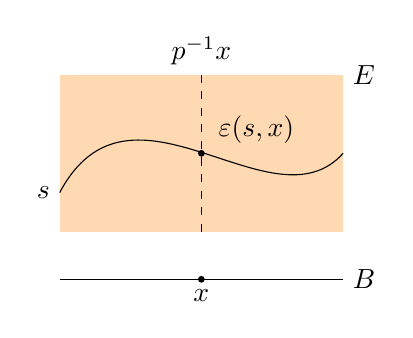
\begin{tikzpicture}

    \def\dy{0.2};
    \def\yb{-0.6}; % base
    \def\yfb{0}; % fiber bottom
    \def\yfs{0.5}; % s
    \def\yfss{1.0}; % s'
    \def\yft{2}; % fiber top

    \def\dx{0.9};

    \def\xbl{0};
    \def\xbmr{\xbl + 2*\dx};
    \def\xbr{\xbl + 4*\dx};

    \filldraw[fill=orange!30, draw=white] (\xbl, \yfb) rectangle (\xbr, \yft);

    \draw (\xbl, \yfb+0.5) .. controls (\xbl + \dx, \yfb + 2.2) and (\xbl + 3* \dx, \yfb) .. (\xbr, \yfb + 1);
    \filldraw[black] (\xbmr, \yfb + 1) circle (1 pt);
    \node[ above] at (\xbmr + 0.7, \yfb + 1) {$\varepsilon(s, x)$};
    \node[left] at  (\xbl, \yfb+0.5) {$s$};
    \draw (\xbl, \yb) -- (\xbr, \yb);

    \draw[dashed] (\xbmr, \yfb) -- (\xbmr, \yft); %fiber


    \filldraw[black] (\xbmr, \yb) circle (1 pt);
    \node[below] at (\xbmr, \yb) {$x$};

    \node[above] at (\xbmr, \yft) {$p^{-1} x$};

    \node[right] at (\xbr, \yb) {$B$};
    \node[right] at (\xbr, \yft) {$E$};

   \end{tikzpicture}
  \]
  换句话说,该图必须交换:
  \[
   \begin{tikzcd}
    S(E) \times B
    \arrow[rr, "\varepsilon"]
    \arrow[dr, "\pi_2"']
    && E
    \arrow[dl, "p"]
    \\
    &B
   \end{tikzcd}
  \]
  这使得 $\varepsilon$ 成为商范畴 $\mathcal{C}/B$ 中的一个态射。

  正如我们定义了函数对象的普遍性一样,截面对象也是普遍的。普遍性条件具有相同的形式:对于任何其他具有箭头 $\phi \colon G \times B \to E$ 的对象 $G$,存在一个唯一的箭头 $\phi^T \colon G \to S(E)$ 使得以下图表交换:
  \[
   \begin{tikzcd}
    G \times B
    \arrow[d, dashed, "\phi^T \times B"']
    \arrow[dr, "\phi"]
    \\
    S(E) \times B
    \arrow[r, "\varepsilon"]
    &E
   \end{tikzcd}
  \]
  不同之处在于 $\varepsilon$ 和 $\phi$ 现在都是商范畴 $\mathcal{C}/B$ 中的态射。

  $\phi$ 和 $\phi^T$ 之间的一一对应关系形成了伴随关系:
  \[(\mathcal{C}/B) \left( \left \langle {G\times B \atop \pi_2} \right \rangle , \left \langle {E \atop p } \right \rangle \right) \cong \mathcal{C} \left(G, S(E)\right) \]
  我们可以用它作为截面对象 $S(E)$ 的定义。这个伴随关系的余单元是依赖函数的应用。我们通过用 $S(E)$ 替换 $G$ 并在右侧选择恒等态射来获得它。余单元因此成为同态集的一个成员:
  \[(\mathcal{C}/B) \left( \left \langle {S(E) \times B \atop \pi_2} \right \rangle , \left \langle {E \atop p } \right \rangle \right) \]


  将上面的伴随关系与定义函数对象 $E^B$ 的柯里化伴随关系进行比较:
  \[  \cat C (G \times B, E) \cong \cat C (G, E^B) \]

  现在回想一下,在 $\mathbf{Set}$ 中,我们将积 $G \times B$ 解释为在 $B$ 的每个元素上植入 $G$ 的副本。因此,我们的伴随关系的左侧的单个元素是一个函数族,每个纤维一个函数。给定 $G$ 中的任意一个 $y$,它在 $G \times B$ 中切出一个水平切片。这些是所有 $b \in B$ 的对 $(y, b)$。我们的函数族将这个切片映射到 $E$ 的对应纤维中,从而创建一个 $E$ 的截面。

  \[
   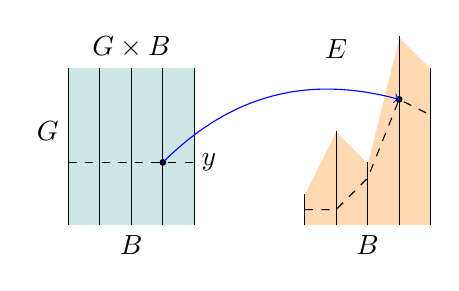
\begin{tikzpicture}
    \def\dy{0.2};
    \def\yb{0};
    \def\yt{10 * \dy};

    \def\dx{0.4};
    \def\xl{-2};
    \def\xr{1};

    \filldraw[fill=blue!50!green!20, draw=white] (\xl, \yb) rectangle (\xl + 4 * \dx, \yt);
    \draw (\xl, \yb) -- (\xl, \yt);
    \draw (\xl + \dx, \yb) -- (\xl + \dx, \yt);
    \draw (\xl + 2 * \dx, \yb) -- (\xl + 2 * \dx, \yt);
    \draw (\xl + 3 * \dx, \yb) -- (\xl + 3 * \dx, \yt);
    \draw (\xl + 4 * \dx, \yb) -- (\xl + 4 * \dx, \yt);
    \node[below] at (\xl + 2 * \dx, \yb) {$B$};
    \node[left] at (\xl + 5 * \dx,  4 * \dy) {$y$};
    \node[left] at (\xl,  6 * \dy) {$G$};
    \node[above] at (\xl + 2*\dx, 10 * \dy) {$G \times B$};

    \def\a{2* \dy}
    \def\b{6* \dy}
    \def\c{4* \dy}
    \def\d{12* \dy}
    \def\e{10* \dy}


    \draw[fill=orange!30, draw=white] (\xr, \yb) -- (\xr, \a) -- (\xr + 1 * \dx, \b) -- (\xr + 2 * \dx, \c) -- (\xr + 3 * \dx, \d) -- (\xr + 4 * \dx, \e) -- (\xr + 4 * \dx, \yb) -- cycle;


    \draw (\xr, \yb) -- (\xr, \a);
    \draw (\xr + \dx, \yb) -- (\xr + \dx, \b);
    \draw (\xr + 2 * \dx, \yb) -- (\xr + 2 * \dx, \c);
    \draw (\xr + 3 * \dx, \yb) -- (\xr + 3 * \dx, \d);
    \draw (\xr + 4 * \dx, \yb) -- (\xr + 4 * \dx, \e);

    \node[below] at (\xr + 2 * \dx, \yb) {$B$};
    \node[above] at (\xr + \dx, 10 * \dy) {$E$};

    \draw[dashed] (\xr, \a -\dy ) -- (\xr + 1 * \dx, \b - 5 * \dy) -- (\xr + 2 * \dx, \c - \dy) -- (\xr + 3 * \dx, \d - 4*\dy) -- (\xr + 4 * \dx, \e - 3*\dy);


    \filldraw[black] (\xl + 3 * \dx, \yb + 4* \dy) circle (1 pt);
    \filldraw[black] (\xr + 3 * \dx, \yb + 8* \dy) circle (1 pt);

    \draw[blue] ((\xl + 3 * \dx, \yb + 4* \dy) edge[->, bend left] (\xr + 3 * \dx, \yb + 8* \dy);

    \draw[dashed] (\xl, \yb + 4* \dy) -- (\xl + 4* \dx, \yb + 4* \dy);

   \end{tikzpicture}
  \]

  伴随关系告诉我们,这些映射族唯一地确定了从 $G$ 到 $S(E)$ 的函数。因此,$S(E)$ 的元素与 $E$ 的截面一一对应。

  这些都是集合论的直觉。我们可以通过首先注意到伴随关系的右侧可以很容易地表达为终对象上商范畴 $\mathcal{C}/1$ 中的同态集来推广它们。

  确实,$\mathcal{C}$ 中的对象 $X$ 和 $\mathcal{C}/1$ 中的对象 $\langle X, ! \rangle$ 之间存在一一对应关系(这里 $!$ 是指向终对象的唯一箭头)。$\mathcal{C}/1$ 中的箭头是 $\mathcal{C}$ 中的箭头,没有额外的约束。因此,我们有:
  \[(\mathcal{C}/B) \left( \left \langle {G\times B \atop \pi_2} \right \rangle , \left \langle {E \atop p } \right \rangle \right) \cong (\mathcal{C}/1)  \left( \left \langle {G \atop !} \right \rangle , \left \langle {S(E) \atop ! } \right \rangle \right)  \]

  \subsection{添加图集 (Adding the atlas)}

  下一步是通过用更一般的基 $A$ 代替终对象 $1$ 来“模糊焦点”,$A$ 作为图集。

  伴随关系的右侧变为商范畴 $\mathcal{C}/A$ 中的同态集。$G$ 本身通过某种 $q \colon G \to A$ 进行粗略纤维化。

  请记住,$G \times B$ 可以理解为沿映射 $! \colon B \to 1$ 的拉回,或从 $1$ 到 $B$ 的基变换。如果我们想用 $A$ 替换 $1$,我们应该用更一般的 $q$ 的拉回代替积 $G \times B$。这种基变换由一个新的态射 $f \colon B \to A$ 参数化。

  \[
   \begin{tikzcd}
    G \times B
    \arrow[dr, phantom,  , very near start, "\lrcorner"]
    \arrow[d, "\pi_2"]
    \arrow[r, "\pi_1"]
    & G
    \arrow[d, "!"]
    \\
    B
    \arrow[r, "!"]
    &
    1
   \end{tikzcd}
   \hspace{20pt}
   \begin{tikzpicture}
    \draw[->] (0, 0) -- (1, 0);
   \end{tikzpicture}
   \hspace{20pt}
   \begin{tikzcd}
    f^* G
    \arrow[dr, phantom,  , very near start, "\lrcorner"]
    \arrow[d, "f^*q"']
    \arrow[r, "g"]
    & G
    \arrow[d, "q"]
    \\
    B
    \arrow[r, "f"]
    &A
   \end{tikzcd}
  \]

  结果是,我们得到的不再是 $B$ 上的 $G$ 纤维,而是一个通过 $f^{-1}$ 重新植入 $A$ 中的 $G$ 纤维的拉回 $f^* G$。这样 $A$ 就成了一个图集,它枚举了所有由均匀纤维填充的补丁。

  例如,假设 $A$ 是一个两元素集合。纤维化 $q$ 将 $G$ 分为两个纤维。它们将作为我们的通用纤维。这些纤维现在根据 $f^{-1}$ 的引导重新植入 $B$ 中的两个补丁中,形成 $f^* G$。

  \[
   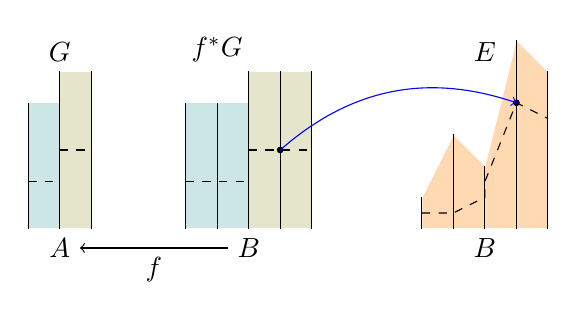
\begin{tikzpicture}
    \def\xmin{-4};

    \def\dy{0.2};
    \def\yb{0};
    \def\yt{10 * \dy};

    \def\dx{0.4};
    \def\xl{-2};
    \def\xr{1};

    \filldraw[fill=blue!50!green!20, draw=white] (\xmin, \yb) rectangle (\xmin + \dx, \yt - 2*\dy);
    \filldraw[fill=red!50!green!20, draw=white] (\xmin + \dx, \yb) rectangle (\xmin + 2 * \dx, \yt);
    \draw (\xmin, \yb) -- (\xmin, \yt - 2*\dy);
    \draw (\xmin + \dx, \yb) -- (\xmin+ \dx, \yt);
    \draw (\xmin + 2 * \dx, \yb) -- (\xmin + 2 * \dx, \yt);
    \node[below] (BB) at (\xmin + \dx, \yb) {$A$};
    \node[above] at (\xmin + \dx, 10 * \dy) {$G$};



    \filldraw[fill=blue!50!green!20, draw=white] (\xl, \yb) rectangle (\xl + 4 * \dx, \yt - 2*\dy);
    \filldraw[fill=red!50!green!20, draw=white] (\xl + 2 * \dx, \yb) rectangle (\xl + 4 * \dx, \yt);
    \draw (\xl + 0 * \dx, \yb) -- (\xl + 0 * \dx, \yt - 2 * \dy);
    \draw (\xl + 1 * \dx, \yb) -- (\xl + 1 * \dx, \yt - 2 * \dy);
    \draw (\xl + 2 * \dx, \yb) -- (\xl + 2 * \dx, \yt);
    \draw (\xl + 3 * \dx, \yb) -- (\xl + 3 * \dx, \yt);
    \draw (\xl + 4 * \dx, \yb) -- (\xl + 4 * \dx, \yt);
    \node[below] (B) at (\xl + 2 * \dx, \yb) {$B$};
    \node[above] at (\xl + \dx, 10 * \dy) {$f^* G$};

    \draw[->]  (B) -- (BB) node [midway, below] {$f$};

    \def\a{2* \dy}
    \def\b{6* \dy}
    \def\c{4* \dy}
    \def\d{12* \dy}
    \def\e{10* \dy}


    \draw[fill=orange!30, draw=white] (\xr, \yb) -- (\xr, \a) -- (\xr + 1 * \dx, \b) -- (\xr + 2 * \dx, \c) -- (\xr + 3 * \dx, \d) -- (\xr + 4 * \dx, \e) -- (\xr + 4 * \dx, \yb) -- cycle;


    \draw (\xr, \yb) -- (\xr, \a);
    \draw (\xr + \dx, \yb) -- (\xr + \dx, \b);
    \draw (\xr + 2 * \dx, \yb) -- (\xr + 2 * \dx, \c);
    \draw (\xr + 3 * \dx, \yb) -- (\xr + 3 * \dx, \d);
    \draw (\xr + 4 * \dx, \yb) -- (\xr + 4 * \dx, \e);

    \node[below] at (\xr + 2 * \dx, \yb) {$B$};
    \node[above] at (\xr + 2 * \dx, 10 * \dy) {$E$};

% dashed zigzag in E
    \draw[dashed] (\xr, \a -\dy ) -- (\xr + 1 * \dx, \b - 5 * \dy) -- (\xr + 2 * \dx, \c - 2* \dy)  -- (\xr + 2 * \dx, \c - \dy) -- (\xr + 3 * \dx, \d - 4*\dy) -- (\xr + 4 * \dx, \e - 3*\dy);

    \filldraw[black] (\xl + 3 * \dx, \yb + 5* \dy) circle (1 pt);
    \filldraw[black] (\xr + 3 * \dx, \yb + 8* \dy) circle (1 pt);

% arrow from f*G to E
    \draw[blue] ((\xl + 3 * \dx, \yb + 5* \dy) edge[->, bend left] (\xr + 3 * \dx, \yb + 8* \dy);

% dashed slices through f*G
    \draw[dashed] (\xl, \yb + 3* \dy) -- (\xl + 2 * \dx, \yb + 3* \dy);
    \draw[dashed] (\xl + 2 * \dx, \yb + 5* \dy) -- (\xl + 4* \dx, \yb + 5* \dy);

% slices through G
    \draw[dashed] (\xmin, \yb + 3* \dy) -- (\xmin + \dx, \yb + 3* \dy);
    \draw[dashed] (\xmin + \dx, \yb + 5* \dy) -- (\xmin + 2 * \dx, \yb + 5* \dy);

   \end{tikzpicture}
  \]

  定义依赖函数类型的伴随关系为:
  \[ (\mathcal{C}/B) \left( f^* \left \langle {G \atop q} \right \rangle, \left \langle {E \atop p} \right \rangle \right) \cong  (\mathcal{C}/A)\left( \left \langle {G \atop q} \right \rangle, \Pi_f \left \langle {E \atop p } \right \rangle \right) \]
  这是我们用来定义截面对象 $S(E)$ 的伴随关系的推广。这个定义了一个新对象 $\Pi_f E$,它是截面对象的重新排列。

  伴随关系是在它们各自的商范畴中的映射之间的映射:

  \[
   \begin{tikzcd}
    f^* G
    \arrow[rr, "\phi"]
    \arrow[rd, "f^* q"']
    &&E
    \arrow[dl, "p"]
    \\
    &B
   \end{tikzcd}
   \hspace{20pt}
   \begin{tikzcd}
    G
    \arrow[rr, "\phi^T"]
    \arrow[rd, "q"']
    && \Pi_f E
    \arrow[ld, "\Pi_f \, p"]
    \\
    & A
   \end{tikzcd}
  \]

  为了更好地理解这个伴随关系,让我们考虑它在集合上是如何工作的。

  \begin{itemize}
   \item 右侧在以图集 $A$ 为基的粗粒纤维化中操作。它是一个函数族,每个补丁一个函数。对于每个补丁,我们从 $G$ 的“厚纤维”(下图中为蓝色)到 $\Pi_f E$ 的“厚纤维”(未显示)得到一个函数。

   \item 左侧在以 $B$ 为基的更精细的纤维化中操作。这些纤维分组成小束并覆盖补丁。一旦我们选择一个补丁(下图中为红色),我们就从该补丁到 $E$ 中相应补丁(绿色表示)得到一个函数族——$E$ 中小束的截面。因此,逐个补丁,我们得到 $E$ 的小截面。
  \end{itemize}
  伴随关系告诉我们,$\Pi_f E$ 的“厚纤维”的元素与相同补丁上的 $E$ 的小截面相对应。

  \[
   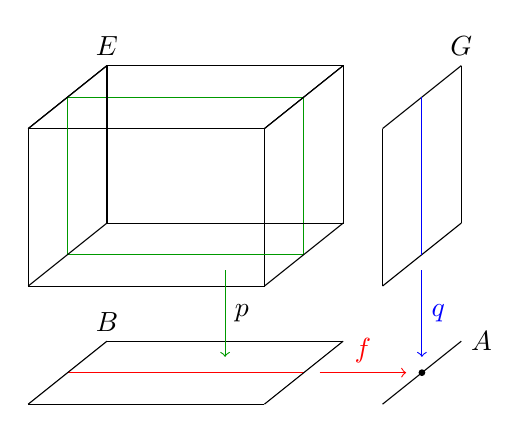
\begin{tikzpicture}
    \def\xl{-3};
    \def\xr{0};
    \def\yb{0};
    \def\yt{2};

    \def\dy{0.4};
    \def\dx{0.5};

    \def\a{(\xl, \yb)};
    \def\b{(\xr, \yb)};
    \def\c{(\xl, \yt)};
    \def\d {(\xr, \yt)};

% _a second plane
    \def\aa{(\xl + \dx, \yb + \dy)};
    \def\ba{(\xr + \dx, \yb + \dy)};
    \def\ca{(\xl + \dx, \yt + \dy)};
    \def\da{(\xr + \dx, \yt + \dy)};

% _b third plane
    \def\ab{(\xl + 2*\dx, \yb + 2*\dy)};
    \def\bb{(\xr + 2*\dx, \yb + 2*\dy)};
    \def\cb{(\xl + 2*\dx, \yt + 2*\dy)};
    \def\db{(\xr + 2*\dx, \yt + 2*\dy)};

% shifted walls
    \def\yshift{-1.5};
    \def\xshift{1.5};


% E
    \draw \a rectangle \d;
    \draw[draw=black!40!green] \aa rectangle \da;
    \draw \ab rectangle \db;

    \draw \a -- \ab;
    \draw \b -- \bb;
    \draw \d -- \db;
    \draw \c -- \cb;

    \node[above] at \cb {$E$};

% B
% rebase yb (bottom)
    \def\yb{\yshift}
% rebase xr (right wall)
    \def\xr{0};

    \draw \a -- \b;
    \draw \ab -- \bb;
    \draw[red] \aa -- \ba;
% diagonal
    \draw \a -- \ab;
    \draw \b -- \bb;
    \draw \d -- \db;
    \draw \c -- \cb;
    \node[above] at \ab {$B$};

% G
% rebase yb (bottom)
    \def\yb{0};
% rebase xr (right wall)
    \def\xr{\xshift};
    \draw \b -- \bb;
    \draw \d -- \db;
    \draw \b -- \d;
    \draw \bb -- \db;
    \draw[blue] \ba -- \da;
    \node[above] at \db {$G$};

% A
% rebase yb (bottom)
    \def\yb{\yshift}
% rebase xr (right wall)
    \def\xr{\xshift};

    \draw \b -- \bb;
    \node[right] at \bb {$A$};
    \filldraw[black] \ba circle (1 pt);

%projections
    \draw[blue, shorten <=0.2cm, shorten >=0.2cm, ->] (\xshift + \dx, 0 + \dy) -- node[right]{$q$} (\xshift +\dx, \yshift + \dy);

    \draw[red, shorten <=0.2cm, shorten >=0.2cm, ->] (0 + \dx, \yshift + \dy) -- node[above]{$f$} (\xshift +\dx, \yshift + \dy);

    \draw[draw=black!40!green, shorten <=0.2cm, shorten >=0.2cm, ->] (0 - \dx, 0 + \dy) -- node[right]{$p$} (0 - \dx, \yshift + \dy);

   \end{tikzpicture}
  \]

  在范畴论中,依赖积是基变换函子 $f^*$ 的右伴随,记作 $f_*$。对于给定的 $f \colon b \to a$,它是一个函子:
  \[ f_* \colon \cat C/b \to \cat C/a \]

  以下练习揭示了 $f$ 所起的作用。它可以被视为通过限制它们在由 $f^{-1}$ 定义的“邻域”上的截面来定位 $E$ 的截面。

  \begin{exercise}
   考虑当 $A$ 是一个两元素集合 $\{0, 1\}$ 并且 $f$ 将整个 $B$ 映射到一个元素(比如 $1$)时会发生什么。你将如何定义伴随关系右侧的函数?它应该对 $0$ 上的纤维做些什么?
  \end{exercise}

  \begin{exercise}
   我们选择 $G$ 为单元素集合 $1$,并让 $x \colon 1 \to A$ 作为一个选择 $A$ 中元素的纤维化。使用伴随关系,证明以下结论:
   \begin{itemize}
    \item $f^* 1$ 有两种类型的纤维:$f^{-1} (x)$ 的元素上的单元集和空集。
    \item 一个映射 $\phi \colon f^* 1 \to E$ 等同于从 $E$ 的每个 $f^{-1}(x)$ 的纤维中选择一个元素。换句话说,它是 $E$ 在 $B$ 的子集 $f^{-1}(x)$ 上的部分截面。
    \item $\Pi_f E$ 的一个纤维是这样的部分截面。
    \item 当 $A$ 也是一个单元素集合时会发生什么?
   \end{itemize}
  \end{exercise}



  \subsection{全称量化 (Universal quantification)}

  依赖积 $\Pi_{x : B} \, T(x)$ 的逻辑解释是一个全称命题。类型 $\Pi_{x : B} \, T(x)$ 的一个元素是一个截面——它证明了可以从 $T(x)$ 的每个成员中选择一个元素。这意味着它们都不是空的。换句话说,它是命题的证明:
  \[ \forall_{x : B}\, T(x) \]

\section{Equality}

Our first experience in mathematics involves equality. We learn that 
\[1+1=2\] 
and we don't think much of it afterwards. 

But what does it mean that $1+1$ is equal to $2$? Two is a number, but one plus one is an expression, so they are not the same thing. There is some mental processing that we have to perform before we pronounce these two things equal. 

Contrast this with the statement $0 = 0$, in which both sides of equality are \emph{the same thing}. 

It makes sense that, if we are to define equality, we'll have to at least make sure that everything is equal to itself. We call this property \emph{reflexivity}. 

Recall our definition of natural numbers:
\begin{haskell}
data Nat where
  Z :: Nat
  S :: Nat -> Nat
\end{haskell}

This is how we can define equality for natural numbers:
\begin{haskell}
equal :: Nat -> Nat -> Bool
equal Z Z = True
equal (S m) (S n) = equal m n
equal _ _ = False
\end{haskell}
We are recursively stripping $S$'s in each number until one of them reaches $Z$. If the other reaches $Z$ at the same time, we pronounce the numbers we started with to be equal, otherwise they are not. 

\subsection{Equational reasoning}

Notice that, when defining equality in Haskell, we were already using the equal sign. For instance, the equal sign in:
\begin{haskell}
equal Z Z = True
\end{haskell}
tells us that wherever we see the expression \hask{equal Z Z} we can replace it with \hask{True} and vice versa. 

This is the principle of substituting equals for equals, which is the basis for \emph{equational reasoning} in Haskell. We can't encode proofs of equality directly in Haskell, but we can use equational reasoning to reason about Haskell programs. This is one of the main advantages of pure functional programming. You can't perform such substitutions in imperative languages, because of side effects.

If we want to prove that $1+1$ is $2$, we have to first define addition. The definition can either be recursive in the first or in the second argument. This one recurses in the second argument:
\begin{haskell}
add :: Nat -> Nat -> Nat
add n Z = n
add n (S m) = S (add n m)
\end{haskell}
We encode $1 + 1$ as:
\begin{haskell}
add (S Z) (S Z)
\end{haskell}
We can now use the definition of \hask{add} to simplify this expression. We try to match the first clause, and we fail, because \hask{S Z} is not the same as \hask{Z}. But the second clause matches. In it, \hask{n} is an arbitrary number, so we can substitute \hask{S Z} for it, and get:
\begin{haskell}
add (S Z) (S Z) = S (add (S Z) Z)
\end{haskell}
In this expression we can perform another substitution of equals using the first clause of the definition of \hask{add} (again, with \hask{n} replaced by \hask{S Z}):
\begin{haskell}
add (S Z) Z = (S Z)
\end{haskell}
We arrive at:
\begin{haskell}
add (S Z) (S Z) = S (S Z)
\end{haskell}
We can clearly see that the right-hand side is the encoding of $2$. But we haven't shown that our definition of equality is reflexive so, in principle, we don't know if
\begin{haskell}
eq (S (S Z)) (S (S Z))
\end{haskell}
yields \hask{True}. We have to use step-by-step equational reasoning again:
\begin{haskell}
equal (S (S Z) (S (S Z)) =
{- second clause of the definition of equal -}
equal (S Z) (S Z) =
{- second clause of the definition of equal -}
equal Z Z =
{- first clause of the definition of equal -}
True
\end{haskell}

We can use this kind of reasoning to prove statements about concrete numbers, but we run into problems when reasoning about generic numbers---for instance, showing that something is true for all \hask{n}. Using our definition of addition, we can easily show that \hask{add n Z} is the same as \hask{n}. But we can't prove that \hask{add Z n} is the same as \hask{n}. The latter proof requires the use of induction. 

We end up distinguishing between two kinds of equality. One is proven using substitutions, or rewriting rules, and is called \emph{definitional equality}. You can think of it as macro expansion or inline expansion in programming languages. It also involves $\beta$-reductions: performing function application by replacing formal parameters by actual arguments, as in:
\begin{haskell}
(\x -> x + x) 2 =
{- beta reduction -}
2 + 2
\end{haskell}

The second more interesting kind of equality is called \emph{propositional equality} and it may require actual proofs. 

\subsection{Equality vs isomorphism}

We said that category theorists prefer isomorphism over equality---at least when it comes to objects. It is true that, within the confines of a category, there is no way to differentiate between isomorphic objects. In general, though, equality is stronger than isomorphism. This is a problem, because it's very convenient to be able to substitute equals for equals, but it's not always clear that one can substitute isomorphic for isomorphic. 

Mathematicians have been struggling with this problem, mostly trying to modify the definition of isomorphism---but a real breakthrough came when they decided to simultaneously weaken the definition of equality. This led to the development of \emph{homotopy type theory}, or HoTT for short. 

Roughly speaking, in type theory, specifically in Martin-L{\"o}f theory of dependent types, equality is represented as a type, and in order to prove equality one has to construct an element of that type---in the spirit of the Curry-Howard interpretation. 

Furthermore, in HoTT, the proofs themselves can be compared for equality, and so on ad infinitum. You can picture this by considering proofs of equality not as points but as some abstract paths that can be morphed into each other; hence the language of homotopies.

In this setting, instead of isomorphism, which involves strict equalities of arrows:
\[ f \circ g = id \]
\[ g \circ f = id \]
one defines an \emph{equivalence}, in which these equalities are treated as types.

The main idea of HoTT is that one can impose the \emph{univalence axiom} which, roughly speaking, states that equalities are equivalent to equivalences, or symbolically:
\[ (A = B) \cong (A \cong B) \]
Notice that this is an axiom, not a theorem. We can either take it or leave it and the theory is still valid (at least we think so).
\subsection{Equality types}

Suppose that you want to compare two terms for equality. The first requirement is that both terms be of the same type. You can't compare apples with oranges. Don't get confused by some programming languages allowing comparisons of unlike terms: in every such case there is an implicit conversion involved, and the final equality is always between same-type values. 

For every pair of values there is, in principle, a separate type of proofs of equality. There is a type for $0 = 0$, there is a type for $1=1$, and there is a type for $1 = 0$; the latter hopefully uninhabited. 

Equality type, a.k.a., identity type, is therefore a dependent type: it depends on the two values that we are comparing. It's usually written as $\mathit{Id}_A$, where $A$ is the type of both values, or using an infix notation as $x=_A y$ (equal sign with the subscript $A$). 

For instance, the type of equality of two zeros is written as $\mathit{Id}_{\mathbb{N}} (0, 0)$ or:
\[ 0 =_{\mathbb{N}} 0 \]
Notice: this is not a statement or a term. It's a \emph{type}, like \hask{Int} or \hask{Bool}. You can define a value of this type if you have an introduction rule for it.

\subsection{Introduction rule}

The introduction rule for the equality type is the dependent function: 
\[ \mathit{refl}_A \colon \Pi_{x : A}  \mathit{Id}_A  (x, x)\]
which can be interpreted in the spirit of propositions as types as the proof of the statement:
\[ \forall _{x:A} \;x = x \]
This is the familiar reflexivity: it shows that, for all $x$ of type $A$, $x$ is equal to itself. You can apply this function to some concrete value $x$ of type $A$, and it will produce a new value of type $\mathit{Id}_A  (x, x)$.

We can now prove that $0=0$. We can execute $\mathit{refl}_{\mathbb{N}} (0)$ to get a value of the type $0 =_{\mathbb{N}} 0$. This value is the proof that the type is inhabited, and therefore corresponds to a true proposition.

This is the only introduction rule for equality, so you might think that all proofs of equality boil down to ``they are equal because they are the same.'' Surprisingly, this is not the case. 

\subsection{$\beta$-reduction and $\eta$-conversion}

In type theory we have this interplay of introduction and elimination rules that essentially makes them the inverse of each other. 

Consider the definition of a product. We introduce it by providing two values, $x \colon A$ and $y \colon B$ and we get a value $p \colon A \times B$. We can then eliminate it by extracting two values using two projections. But how do we know if these are the same values that we used to construct it? This is something that we have to postulate. We call it the computation rule or the $\beta$-reduction rule.

Conversely, if we are given a value $p \colon A \times B$, we can extract the two components using projections, and then use the introduction rule to recompose it. But how do we know that we'll get the same $p$? This too has to be postulated. This is sometimes called the uniqueness condition, or the $\eta$-conversion rule.

In the categorical model of type theory these two rules follow from the universal construction. 

The equality type also has the elimination rule, which we'll discuss shortly, but we don't impose the uniqueness condition. It means that it's possible that there are some equality proofs that were not obtained using $\mathit{refl}$. 

This is exactly the weakening of the notion of equality that makes HoTT interesting to mathematicians.

\subsection{Induction principle for natural numbers}

Before formulating the elimination rule for equality, it's instructive to first discuss a simpler elimination rule for natural numbers. We've already seen such rule describing primitive recursion. It allowed us to define recursive functions by specifying a value $\mathit{init}$ and a function $\mathit{step}$.

Using dependent types, we can generalize this rule to define the \emph{dependent elimination rule} that is equivalent to the principle of mathematical induction.

The principle of induction can be described as a device to prove, in one fell swoop, whole families of propositions indexed by natural numbers. For instance, the statement that \hask{add Z n} is equal to \hask{n} is really an infinite number of propositions, one per each value of \hask{n}. 

We could, in principle, write a program that would meticulously verify this statement for a very large number of cases, but we'd never be sure if it holds in general. There are some conjectures about natural numbers that have been tested this way using computers but, obviously, they can never exhaust an infinite set of cases.

Roughly speaking, we can divide all mathematical theorems into two groups: the ones that can be easily formulated and the ones whose formulation is complex. They can be further subdivided into the ones whose proofs are simple, and the ones that are hard or impossible to prove. For instance, the famous Fermat's Last Theorem was extremely easy to formulate, but its proof required some massively complex mathematical machinery. 

Here, we are interested in theorems about natural numbers that are both easy to formulate and easy to prove. We'll assume that we know how to generate a family of propositions or, equivalently, a dependent type $T(n)$, where $n$ is a natural number. 

We'll also assume that we have a value:
\[\mathit{init} \colon T(Z) \]
or, equivalently, the proof of the zeroth proposition; and a dependent function:
\[\mathit{step} \colon \Pi_{n:\mathbb{N}}\,\left(T(n) \to T(S n)\right) \]
This function is interpreted as generating a proof of the $(n + 1)$st proposition from the proof of the $n$th proposition.

The \emph{dependent elimination rule} for natural numbers postulates that, given such $\mathit{init}$ and $\mathit{step}$, there exists a dependent function:
\[f \colon \Pi_{n:\mathbb{N}} \, T(n) \]
This function is interpreted as providing the proof that $T(n)$ is true for all $n$.

Moreover, this function, when applied to zero reproduces $\mathit{init}$:
\[ f (Z) = \mathit{init} \]
and, when applied to the successor of $n$, is consistent with taking a $\mathit{step}$:
\[ f (S n) = (\mathit{step} (n)) (f (n)) \]
(Here, $\mathit{step}(n)$ produces a function, which is then applied to the value $f(n)$.) These are the two \emph{computation rules} for natural numbers. 

Notice that the induction principle is not a theorem about natural numbers. It's part of the \emph{definition} of the type of natural numbers. 

Not all dependent mappings out of natural numbers can be decomposed into $\mathit{init}$ and $\mathit{step}$, just as not all theorems about natural numbers can be proven inductively. There is no $\eta$-conversion rule for natural numbers.

\subsection{Equality elimination rule}

The elimination rule for equality type is somewhat analogous to the induction principle for natural numbers. There we used $\mathit{init}$ to ground ourselves at the start of the journey, and $\mathit{step}$ to make progress. The elimination rule for equality requires a more powerful grounding, but it doesn't have a $\mathit{step}$. There really is no good analogy for how it works, other than through a leap of faith.

The idea is that we want to construct a mapping \emph{out} of the equality type. But since equality type is itself a two-parameter family of types, the mapping out should be a dependent function. The target of this function is another family of types:
\[T(x, y, p)\]
 that depends on the pair of values that are being compared $x, y \colon A$, and the proof of equality $p \colon \mathit{Id}(x, y)$.
 
 The function we are trying to construct is:
 \[ f \colon \Pi_{x, y : A} \Pi_{p : \mathit{Id}(x, y)} \, T(x, y, p) \]

It's convenient to think of it as generating a proof that for all points $x$ and $y$, and for every proof that the two are equal, the proposition $T(x, y, p)$ is true. Notice that, potentially, we have a different proposition for \emph{every proof} that the two points are equal.

The least that we can demand from $T(x, y, p)$ is that it should be true when $x$ and $y$ are literally the same, and the equality proof is the obvious $\mathit{refl}$. This requirement can be expressed as a dependent function:
\[t \colon \Pi_{x : A} \,T\left(x, x, \mathit{refl}(x)\right)\]
Notice that we are not even considering proofs of $x = x$, other than those given by reflexivity. Do such proofs exist? We don't know and we don't care.

So this is our grounding, the starting point of a journey that should lead us to defining our $f$ for all pairs of points and all proofs of equality. The intuition is that we are defining $f$ as a function on a plane $(x, y)$, with a third dimension given by $p$. To do that, we're given something that's defined on the diagonal $(x, x)$, with $p$ restricted to $\mathit{refl}$.

\[
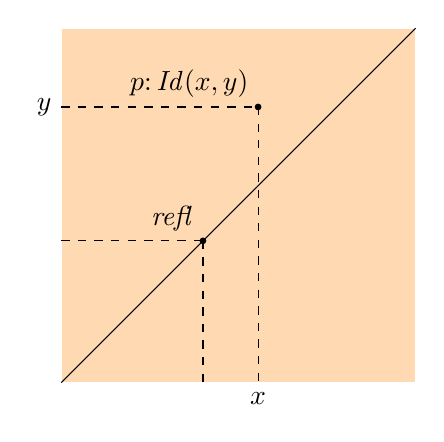
\begin{tikzpicture}

\def\yb{0}; 
\def\ydiag{1.8};
\def\yoff{3.5};
\def\yt{4.5}; 


\def\xl{0};
\def\xdiag{\ydiag};
\def\xoff{2.5};
\def\xr{\yt};

\filldraw[fill=orange!30, draw=white] (\xl, \yb) rectangle (\xr, \yt);

\draw (\xl, \yb) -- (\xr, \yt); % diagonal

\draw[dashed] (\xdiag, \ydiag) -- (\xdiag, \yb);
\draw[dashed] (\xl, \ydiag) -- (\xdiag, \ydiag);

\filldraw[black] (\xdiag, \ydiag) circle (1 pt);
\node[above left] at (\xdiag, \ydiag) {$\mathit{refl}$};

\draw[dashed] (\xoff, \yoff) -- (\xoff, \yb);
\draw[dashed] (\xl, \yoff) -- (\xoff, \yoff);

\filldraw[black] (\xoff, \yoff) circle (1 pt);
\node[above left] at (\xoff, \yoff) {$p\colon \mathit{Id}(x, y)$};

\node[below] at (\xoff, \yb) {$x$};
\node[left] at (\xl, \yoff) {$y$};

\end{tikzpicture}
\]

You would think that we need something more, some kind of a $\mathit{step}$ that would move us from one point to another. But, unlike with natural numbers, there is no \emph{next} point or \emph{next} equality proof to jump to. All we have at our disposal is the function $t$ and nothing else. 

Therefore we postulate that, given a type family $T(x, y, p)$ and a function:
\[t \colon \Pi_{x : A} \,T\left(x, x, \mathit{refl}(x)\right)\]
there exists a function:
 \[ f \colon \Pi_{x, y : A} \Pi_{p : \mathit{Id}(x, y)} \, T(x, y, p) \]
such that (computation rule):
\[f (x, x, \mathit{refl}(x)) = t(x)\]
Notice that the equality in the computation rule is \emph{definitional equality}, not a type.

Equality elimination tells us that it's always possible to extend the function $t$, which is defined on the diagonal, to the whole 3-d space. 

This is a very strong postulate. One way to understand it is to argue that, within the framework of type theory---which is formulated using the language of introduction and elimination rules, and the rules for manipulating those---it's \emph{impossible} to define a type family $T(x, y, p)$ that would \emph{not} satisfy the equality elimination rule. 

The closest analogy that we've seen so far is the result of parametricity, which states that, in Haskell, all polymorphic functions between endofunctors are automatically natural transformations. Another example, this time from calculus, is that any analytic function defined on the real axis has a unique extension to the whole complex plane. 

The use of dependent types blurs the boundary between programming and mathematics. There is a whole spectrum of languages,  starting with Haskell barely dipping its toes in dependent types while still firmly established in commercial usage, all the way to theorem provers, which are helping mathematicians formalize mathematical proofs.

\end{document}